\documentclass{beamer}
 
\usetheme{metropolis}
\setbeamertemplate{frame numbering}[fraction]
\useoutertheme{metropolis}
\useinnertheme{metropolis}
\usefonttheme{metropolis}
\usecolortheme{spruce}
\setbeamercolor{background canvas}{bg=white}

\usepackage[german]{babel}
\usepackage{german}
\usepackage{graphicx}

\graphicspath{{Schrift/images/}}



\title{Aufbau und Funktionsweise eines Prozessors}
\author{Marco Vogel}
\institute{Hochschule Hof}
\date{\today}

\begin{document}

\begin{frame}
\titlepage
\end{frame}

\begin{frame}
\frametitle{Inhaltsverzeichnis}
\tableofcontents
\end{frame}





%-------------------------------------------------------------------------------
\iffalse
\section{Bin\"are Zahlendarstellung}
\begin{frame}[t]{Bin\"are Zahlendarstellung}
Beispiel: 135d = $\sum\limits_{i=0}^{n-1} a_i * 10^i$
\newline
\par\smallskip
$Z=1*10^2+3*10^1+5*10^0 = 100+30+5 = 135$
\par\smallskip\pause
Dezimal zu Bin\"ar: \centering $135d = 1*2^7+0*2^6+0*2^5+0*2^4+0*2^3+*2^2+1*2^1+1*2^0$\newline
\end{frame}


\begin{frame}[t]{Bin\"are Zahlendarstellung}
Beispiel: 135d = $\sum\limits_{i=0}^{n-1} a_i * 10^i$
\newline
\par\smallskip
$Z=1*10^2+3*10^1+5*10^0 = 100+30+5 = 135$
\par\smallskip
Dezimal zu Bin\"ar:\centering\\ $135d = \textbf{1}*2^7+\textbf{0}*2^6+\textbf{0}*2^5+\textbf{0}*2^4+\textbf{0}*2^3+\textbf{1}*2^2+\textbf{1}*2^1+\textbf{1}*2^0$\newline \par\smallskip\pause
$  = 10000111b$\centering
\end{frame}

\fi
%-------------------------------------------------------------------------------




\section{Komponenten eines Prozessors}
\begin{frame}{Komponenten eines Prozessors}
\begin{enumerate}
\large\item{Steuerwerk}\smallskip
\item{Rechenwerk}\smallskip
\item{Registerwerk}\smallskip
\item{Bussystem}\smallskip
\end{enumerate}
\end{frame}

\subsection{Steuerwerk}
\begin{frame}{Steuerwerk}

\end{frame}



\subsection{Rechenwerk}
\begin{frame}{Rechenwerk}

\end{frame}


\subsection{Registerwerk}
\begin{frame}{Registerwerk}
\end{frame}

\subsection{Bussystem}
\begin{frame}{Bussystem}

\end{frame}

\section{Befehlsverarbeitung}
\begin{frame}{Von-Neumann-Zyklus}
\begin{enumerate}\pause
\item{Befehlsabruf}\pause
\item{Dekodierung}\pause
\item{Operandenabruf}\pause
\item{Befehlsausf\"uhrung}\pause
\item{Zur\"uckschreiben des Ergebnisses}
\end{enumerate}
\end{frame}

\section{Planung eines Prozessors}

\begin{frame}[t]{Planung eines Prozessors}
\begin{enumerate}
\item{Bestimmung der zu verwendenden Wortl\"ange}
\end{enumerate}
32 Bit : 00000000000000000000000000000000
\centering 
\pause
\begin{table}[]
\centering
\begin{tabular}{|c|c|c|}
\hline
00000000 & 00000000 & 0000000000000000 \\ \hline
Opcode   & Argument & Value            \\ \hline
\end{tabular}
\end{table}
\smallskip
\pause
\centering
\begin{table}[]
\centering
\begin{tabular}{|c|c|c|c|}
\hline
00000000 & 00000000 & 00000000 & 00000000 \\ \hline
Opcode   & Argument & Ziel     & Quelle   \\ \hline
\end{tabular}
\end{table}
\end{frame}

\begin{frame}[t]{2. Befehlssatz erstellen}\pause
Befehlsarten:
\bigskip
\center
\begin{enumerate}
\item{Transferbefehle  (MOV,XCHG)}
\item{ALU-Befehle \ \ \ (ADD,AND)}
\item{Sprungbefehle  \  (JUMP,CALL)}
\item{Stack-Befehle \ (PUSH,POP)}
\end{enumerate}
\end{frame}

\section{Praxis}
\begin{frame}{Logisim}
Aufbau eines Prozessors in Logisim
\begin{figure}[!htb]
\centering
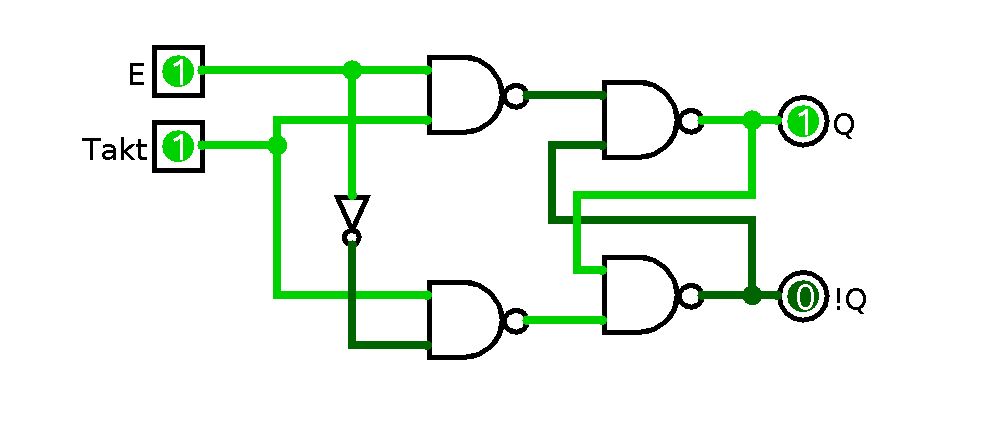
\includegraphics[scale=0.30]{flipflop}
\end{figure}
\end{frame}
\end{document}